\subsection{Rotating Wave Approximation and Rabi oscillations}

We turn our attention now back to the full Hamiltonian of the problem. Let's re-write this equation in a more convinient way:

\begin{equation} \label{mod_ham}
    \hat{\mathcal{H}} = - \frac {\hbar \omega_{L}}{2} \hat{\sigma_{z}} + \hbar \Delta \hat{\Phi} + \hbar \Omega_{R} (e^{i\omega_{L}t} + e^{-i\omega_{L}t}) \hat{\sigma}_{x},
\end{equation}

where $\Delta = \omega_{a} - \omega_{L}$ and $\hat{\Phi} = \ket{1}\bra{1}$. we also shifted the whole energy spectrum by $\hbar \Delta \hat{\mathbb{1}}/2$. Now we write down the transformation to the interaction picture with respect to the first term of expression \ref{mod_ham}, i.e. $\mathcal{H}_{0} = - \frac {\hbar \omega_{L}}{2}$.

Performing the transformation term by term, given that $[\sigma_{z}, \hat{\phi}] = 0$, the first term is symmetrical under the interaction picture transformation. We calculate then how $\hat{\sigma_{x}}$ transforms. Let's write $\hat{\sigma_{x}} = \hat{\sigma^{+}} + \hat{\sigma^{-}}$ and using the baker-Hausdorff lemma:

\begin{equation}
    e^{B}Ae^{-B} = B + [B,A] + \frac{1}{2!} [B, [B,A]] + ...,
\end{equation}

we find:

\begin{equation}
\begin{cases}
    \sigma^{+}_{I} = e^{ i \omega_{L}t} \sigma^{+} \\
    \sigma^{-}_{I} = e^{ - i \omega_{L}t} \sigma^{-}
\end{cases}
\end{equation}

Writing the interaction Hamiltonian in the interaction picture:

\begin{equation}
    \mathcal{H}_{int}^{I} = \hbar \Delta \hat{\phi} + \hbar\Omega_{R} (e^{i \omega_{L} t} + c.c.) (e^{i \omega_{L} t} \hat{\sigma}^{+} + e^{-i \omega_{L} t}\hat{\sigma}^{-})
\end{equation}

In this expression some terms do not oscillate and other oscillate with $2\omega_{L}$. The rotating wave approximation consists in neglecting those fast oscillating terms. The interaction then is finally written:

\begin{equation}
    \mathcal{H}_{int}^{I} = \hbar \Delta \hat{\phi} + \hbar\Omega_{R} \hat{\sigma}_{x}
\end{equation}

In the matrix form, in units of $\hbar$:

\[
\mathcal{H}_{int}^{I} =
  \begin{bmatrix}
    0 & \Omega_{R}  \\
    \Omega_{R} & \Delta
  \end{bmatrix}
\]

Inserting this operator in the TDSE in the interaction picture we find:

\begin{equation} \label{coupled_equations}
\begin{cases}
    i \dot{c}_{0}(t) = \Omega_{R} \dot{c}_{1}(t) \\
    \\
    i \dot{c}_{1}(t) = \Delta c_{1}(t) + \Omega_{R} c_{0}(t),
\end{cases}
\end{equation}
which leads, for the excited state, a general function of the type:

\begin{equation} \label{c1}
    c_{1}(t) = A e^{-i\Delta t / 2}(e^{i\Omega't/2} - e^{-i\Omega't/2}),
\end{equation}

with $\Omega' = \sqrt{\Delta^{2} + 4 \Omega_{R}^{2}}$. This expression was written by having in mind the initial condition $|c_{1}(t=0)|^{2} = 0$, but that is not enough the determine $A$. To determine this coefficient we insert \ref{c1} in the coupled differential equations \ref{coupled_equations}, calculate $c_{0}(t)$ and consider $|c_{0}(t=0)|^{2} = 1$, which fully determines $A$:

\begin{equation}
    \begin{cases}
    |c_{1}(t)|^{2} = \frac{4\Omega_{R}^{2}}{\Delta^{2} + 4 \Omega_{R}^{2}} \frac{1}{2}(1 - \textrm{cos} \Omega't) \\
    \\
    |c_{0}(t)|^{2} = \frac{\Delta^{2}} {\Omega'^{2}} \textrm{sin}^{2}(\Omega't/2) + \textrm{cos}^{2}(\Omega't/2)
    \end{cases}
\end{equation}

The on resonance case $\Delta=0$, flips the population entirely from the ground state to the excited state when the atoms are illuminated with a pulse duration $t_{\pi}$, where $2\Omega_{R}t_{\pi} = \pi$. This is traditionally called a $\pi$--pulse. On figure \ref{rabi_osc} the several cases of pulse duration and detuning are plotted. It is important to note that the $\pi$--pulse value is representative of the dipole matrix connecting the ground and excited states and the laser intensity. Therefore, it is a special property of the atom----laser interaction. Indeed:

\begin{equation}
    \begin{cases}
        \Omega_{R} = \frac{e\mathcal{E}_{0}}{2\hbar} \bra{1} \vec{r} \cdot \hat{\epsilon} \ket{0} \\
        \\
        t_{\pi} = \frac{\pi}{2\Omega_{R}}
    \end{cases}
\end{equation}

\begin{figure}[h]
\centering
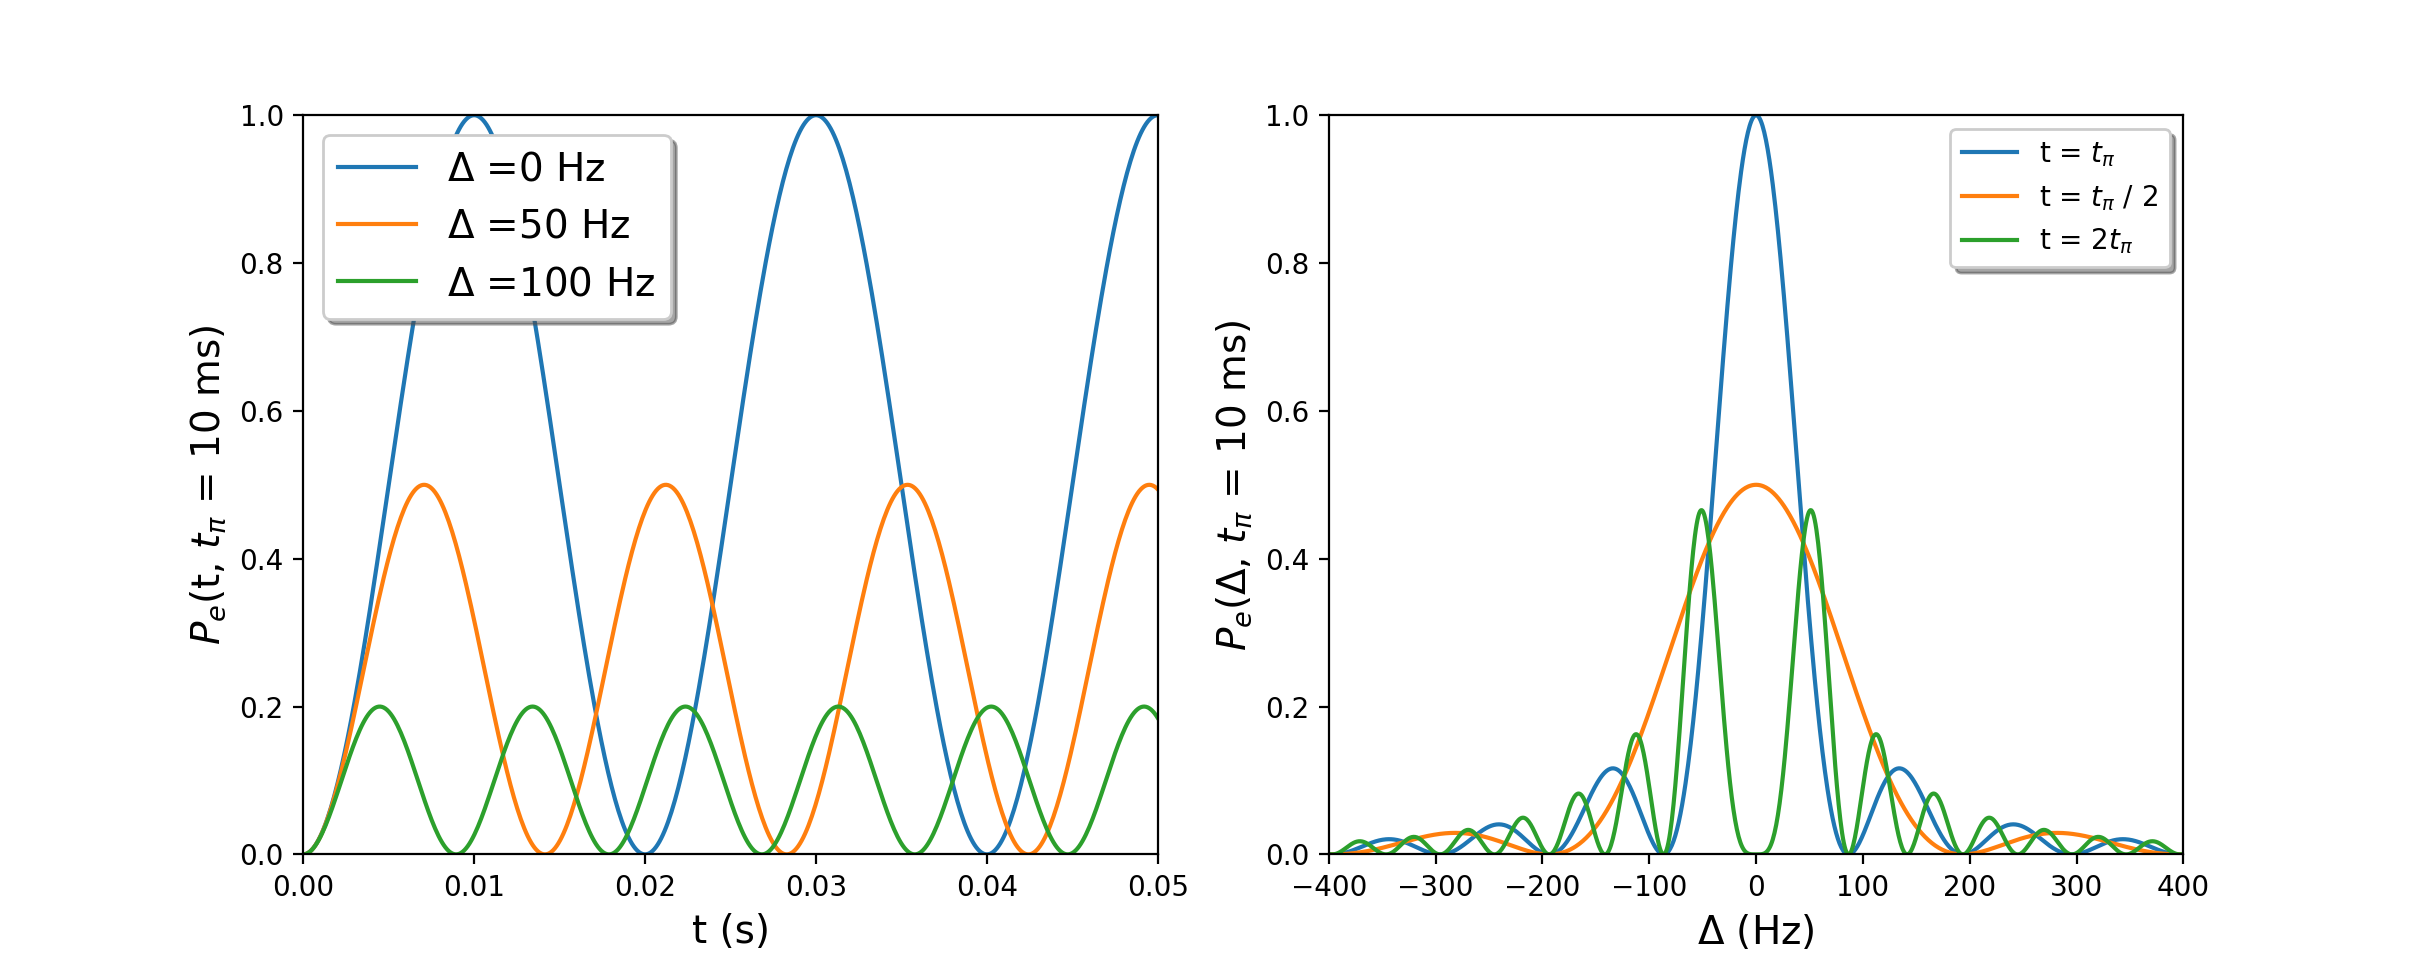
\includegraphics[width=\linewidth]{./plots/Rabi_Oscillations/rabi.png}
\caption{On the right--hand figure it is plotted the transition line shape as a function of the laser detuning from the atomic resonance for different pulse durations. Fixing now the laser frequency with a certain detuning and varying the interaction time or pulse duration, yields to the plot on the left--hand side.}
\label{rabi_osc}
\end{figure}

As you can guess, in the experiment, there are only two parameters that the experimentalist will be interested in to characterize or set up the experiment: $t_{\pi}$ (or the laser intensity) and $\Delta$. It is useful then to re-write the expression for the population of the excited state as a function of these two parameters:

\begin{equation}
    P_{e}(t, \Delta) = \left(\frac{\pi}{2}\right)^{2} \left( \frac{ \textrm{sin}\Delta' t/t_{\pi}} {\Delta'} \right)^{2},
\end{equation}

with $\Delta' = \frac{\pi}{2} \sqrt{1 + (t_{\pi} \Delta / \pi)^{2}}  $.